\documentclass[12pt]{article}
\usepackage[utf8]{inputenc}
\usepackage{amsmath}
\usepackage{amssymb}
\usepackage{amsthm}
\usepackage{fullpage}
\usepackage{graphicx}
\usepackage{hyperref}
\usepackage{enumitem}
\usepackage{algorithm2e}
\usepackage{float}
%% Sets page size and margins
\usepackage[a4paper,top=2.5cm,bottom=2.5cm,left=2cm,right=2cm]{geometry}


%% Title
\title{
		\vspace{-0.7in}
		\usefont{OT1}{bch}{b}{n}
		\begin{minipage}{3cm}
        \vspace{-0.5in}
    	\begin{center}
    		
\includegraphics[height=3.2cm]{../logo_unam.png}
    	\end{center}
    \end{minipage}\hfill
    \begin{minipage}{10.7cm}

    	\begin{center}
\normalfont \normalsize \textsc{UNIVERSIDAD NACIONAL AUTÓNOMA DE MÉXICO \\ FACULTAD DE CIENCIAS \\ Análisis de Algoritmos } \\
		\huge Tarea 3
    	\end{center}

    \end{minipage}\hfill
    \begin{minipage}{3.2cm}
    \vspace{-0.5in}
    	\begin{center}
    		
\includegraphics[height=3.2cm]{../logo_fc.png}
    	\end{center}
    \end{minipage}

\author{Escobar Gonzalez Isaac Giovani \hspace{1cm} 321336400\\
        Garduño Escobar Kevin Jonathan \hspace{0.5cm} 321070629\\
        Zaldivar Alanis Rodrigo \hspace{2.75cm} 424029605 }
\date{}
}

\begin{document}

\maketitle

\section*{Ejercicio 1}
Considera el siguiente algoritmo:\\
\RestyleAlgo{ruled}
\LinesNumbered
\renewcommand{\algorithmcfname}{Algoritmo}
\begin{algorithm}[H]
    Algoritmo: ordenamientoMisterioso( A, n )\\
    \If{$n == 2 \; \& \; A[0] > A[1]$}{
        intercambiar $A[0] \longleftrightarrow A[1]$\;
    }
    \ElseIf{ $n > 2$ } {
        $m = \lceil 2n/3\rceil$\;
        $ordenamientoMisterioso(A[0 .. m-1])$ \;
        $ordenamientoMisterioso(A[n-m .. n-1])$ \;
        $ordenamientoMisterioso(A[0 .. m-1])$ \;
    }
\end{algorithm}
\begin{itemize}
    \item[1.A] Prueba que el algoritmo es correcto (ordena correctamente la salida)
    \item[1.B] ¿El algoritmo es estable?
    \item[1.C] ¿El algoritmo utiliza es $in$ - place (utiliza memoria constante) ?
    \item[1.D] Realiza el análisis de complejidad de tiempo. Plantea y resuelve la ecuación de recurrencia. Concluye mencionando la complejidad asintótica.
    \item[1.E] Si cambiamos $m = \lceil 2n/3 \rceil$ por $m = \lfloor 2n/3 \rfloor$, ¿el algoritmo aún es correcto? Justifica
\end{itemize}
\section*{Ejercicio 2}
Se tienen dos arreglos $A, B$ de longitudes $m, n$ respectivamente. Diseña un algoritmo de tiempo $O(m + n)$ que construya un arreglo $C$ con los elementos en común entre $A$ y $B$, sin elementos repetidos.
\begin{itemize}
    \item[2.A] Da el pseudocódigo
    \item[2.B] Realiza el análisis de correctitud
    \item[2.C] Realiza el análisis de complejidad en tiempo
    \item[2.D] Realiza el análisis de complejidad en espacio
    \item[2.E] Menciona algunos casos interesantes (incluyendo un mejor y peor caso). Ilustra con ejemplos concretos.
\end{itemize}
\section*{Ejercicio 3}
Supón que tenemos un algoritmo en el cual vamos a utilizar pilas (Stacks) pero no conocemos el máximo de elementos a almacenar. Usando arreglos dinámicos, propón una estrategia para trabajar con pilas.
\begin{itemize}
    \item[3.A] Realiza el análisis de la complejidad de tiempo y espacio para las operaciones de la pila (push, pop)
    \item[3.B] Supón que queremos ahorrar el espacio que no se está utilizando, por lo cual se propone reducir el tamaño máximo de la pila a la mitad, cada que la pila reduzca su tamaño a la mitad de elementos. ¿Cómo se modifica el análisis de complejidad del inciso anterior?
    \item[3.C] ¿Cómo se modificaría las respuestas a los incisos anteriores si en vez de una pila consideramos una cola?
\end{itemize}
\section*{Ejercicio 4}
Investiga en qué consiste el método (o teorema) maestro.\\
Ilustra su aplicación con algunos ejemplos.\\
Nota: NO es necesario presentar la demostración del teorema en esta tarea, pero sí es deseable que la revisen y comenten de manera general.\\
El método maestro proporciona una manera de resolver recurrencias de la forma:
\[
    T(n) = aT\left(n/b\right) + f(n)
\]
con $a \geq 1$ y $b > 1$ constantes, y $f(n)$ una función asintóticamente positiva. Una recurrencia de esta forma caracteriza un algoritmo del tipo "divide y vencerás", en el cual un problema de tamaño $n$ se divide en $a$ subproblemas, cada uno de tamaño $n/b$, los $a$ subproblemas se resuelven recursivamente cada uno en tiempo $T\left(n/b\right)$, y la función $f(n)$ es el tiempo que se tarda en dividir el problema y combinar los resultados de los subproblemas.\\
En el teorema maestro, tenemos además que $T(n)$ está definida en los enteros no negativos por la recurrencia e interpretamos $n/b$ como $\lfloor n/b \rfloor$ o $\lceil n/b \rceil$.\\
Así, $T(n)$ tiene las siguientes cotas asintóticas, los tres casos:
\begin{enumerate}
    \item Si $f(n) = O(n^{\log_b a - \epsilon})$ para alguna constante $\epsilon > 0$, entonces $T(n) = \Theta(n^{\log_b a})$.
    \item Si $f(n) = \Theta(n^{\log_b a})$, entonces $T(n) = \Theta(n^{\log_b a} \lg n)$.
    \item Si $f(n) = \Omega(n^{\log_b a + \epsilon})$ para alguna constante $\epsilon > 0$, y si $af(n/b) \leq cf(n)$ para alguna constante $c < 1$ y para todo $n$ suficientemente grande, entonces $T(n) = \Theta(f(n))$.
\end{enumerate}
En los tres casos se compara la función $f(n)$ con la función $n^{\log_b a}$, intiutivamente, la solución a la recurrencia está determinada por la función mayor.\\
Los casos que tiene el método maestro no cubre todas las posibilidades. Existe una diferencia entre los casos 1 y 2 cuando $f(n)$ es más pequeño que $n^{\log_b a}$ pero no polinomialmente menor, también entre los casos 2 y 3 cuando $f(n)$ es más grande que $n^{\log_b a}$ pero no polinomialmente mayor.\\
En el caso de que $f(n)$ entre en alguno de esos huecos o que la condición de regularidad del caso 3 no se cumpla, el método maestro no es aplicable.\\
Algunos ejemplos:
\begin{enumerate}
    \item \textbf{Merge Sort}\\
    La recurrencia para el algoritmo Merge Sort es:
    \[
        T(n) = 2T\left(n/2\right) + \Theta(n)
    \]
    Aquí, $a = 2$, $b = 2$ y $f(n) = \Theta(n)$. Calculamos $n^{\log_b a} = n^{\log_2 2} = n^1 = n$.\\
    Como $f(n) = \Theta(n)$, entonces, $f(n) = \Theta(n^{\log_b a})$, lo que corresponde al caso 2 del teorema maestro. Por lo tanto, la solución es:
    \[
        T(n) = \Theta(n \lg n)
    \]
    \item \textbf{Algoritmo de Strassen para multiplicación de matrices}\\
    La recurrencia para el algoritmo de Strassen es:
    \[
        T(n) = 7T\left(n/2\right) + \Theta(n^2)
    \]
    Aquí, $a = 7$, $b = 2$ y $f(n) = \Theta(n^2)$. Calculamos $n^{\log_b a} = n^{\log_2 7} \approx n^{2.81}$.\\
    Como $f(n) = \Theta(n^2)$, entonces, $f(n) = O(n^{\log_b a - \epsilon})$ para $\epsilon \approx 0.81$, lo que corresponde al caso 1 del teorema maestro. Por lo tanto, la solución es:
    \[
        T(n) = \Theta(n^{\log_2 7}) \approx \Theta(n^{2.81})
    \]
    \item \textbf{$f(n)$ dominante}\\
    Consideremos la siguiente recurrencia:
    \[
        T(n) = 3T\left(n/4\right) + n \lg n
    \]
    Aquí, $a = 3$, $b = 4$ y $f(n) = n \lg n$. Calculamos $n^{\log_b a} = n^{\log_4 3} \approx n^{0.79}$.\\
    Como $f(n) = \Omega(n^{\log_b a + \epsilon})$ para $\epsilon \approx 0.21$, y si verificamos la condición de regularidad: Para $n$ suficientemente grande, $af(n/b) \leq c f(n)$ para alguna constante $c < 1$.
    \begin{align*}
        af(n/b) = 3f(n/4) &= 3(n/4) \lg(n/4)\\
        &= (3/4)n(\lg n - \lg 4) = (3/4)n \lg n - (3/2)n \lg 4\\
        &\leq (3/4)n \lg n
    \end{align*}
    Con $c = 3/4 < 1$, la condición se cumple. Entonces, por el caso 3 del teorema maestro, la solución es:
    \[
        T(n) = \Theta(n \lg n)
    \]
    \item \textbf{Caso no cubierto por el teorema maestro}\\
    Consideremos la siguiente recurrencia:
    \[
        T(n) = 2T\left(n/2\right) + n \lg n
    \]
    Aquí, $a = 2$, $b = 2$ y $f(n) = n \lg n$. Calculamos $n^{\log_b a} = n^{\log_2 2} = n^1 = n$.\\
    En este caso, $f(n)$ no es polinomialmente menor ni mayor que $n^{\log_b a}$, ya que $f(n) = n \lg n$ crece más rápido que $n$ pero más lento que cualquier $n^{1+\epsilon}$ para $\epsilon > 0$. Por lo tanto, el teorema maestro no es aplicable aquí.
\end{enumerate}
La demostración se divide en dos partes: La primera parte analiza la recurrencia maestra, bajo el supuesto de que $T(n)$ se define solo para potencias exactas de $b > 1$.\\
A su vez, esta parte se divide en tres lemas, el primero reduce la solución de la recurrencia a evaluar una expresión que contiene una suma utilizando la técnica de árbol de recurrencia.\\
El segundo lema determina los límites asintóticos de la suma, en este lema se prueban los tres casos del teorema maestro.\\
El tercer lema es la combinación de los dos lemas anteriores, para demostrar una versión del teorema maestro que se aplica a potencias exactas de $b$, entonces, evalúa la suma del primer lema utilizando los límites asintóticos del segundo lema para los tres casos del teorema maestro.\\
La segunda parte de la demostración analiza las situaciones donde aparecen pisos y techos en la recurrencia, así que esté definida para todos los enteros y no solo las potencias exactas de $b$, obteniendo un límite inferior para la recurrencia con techo y un límite superior para la recurrencia con piso, en esta parte también se utiliza el árbol de recurrencia.
\section*{Ejercicio 5}
Para este problema, considera que un subárbol de un árbol binario es cualquier subgráfo conexo. Un árbol binario es completo sí todos los nodos internos tienen dos hijos y cada hoja tiene exactamente la misma profundidad.\\
Describe un algoritmo para calcular el subárbol completo más grande (mayor número de nodos). El algoritmo debería devolver el nodo (o referencia) al subárbol y la altura correspondiente.
\begin{itemize}
    \item[5.A] Da el pseudocódigo
    \item[5.B] Realiza el análisis de complejidad en tiempo
    \item[5.C] Realiza el análisis de correctitud
\end{itemize}
\begin{figure}[H]
    \centering
    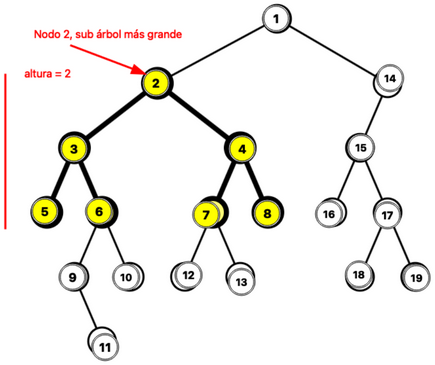
\includegraphics[width=0.7\textwidth]{subárbol.png}
    \caption{Ejemplo de un subárbol binario completo.\\
    En amarillo se indican los nodos correspondientes al subárbol completo más grande.}
\end{figure}

\end{document}
